\documentclass[aspectratio=169]{beamer}
\usepackage{graphicx}
\usepackage{hyperref}
\usetheme{metropolis}
\title{Effective Feedback}
\institute{Engineers for Exploration, UC San Diego}
\logo{
\includegraphics[height=.65cm,keepaspectratio]{e4e_logo_350x136.png}}
\setbeamertemplate{caption}[numbered]
\begin{document}
\maketitle
\begin{frame}
    \centering
    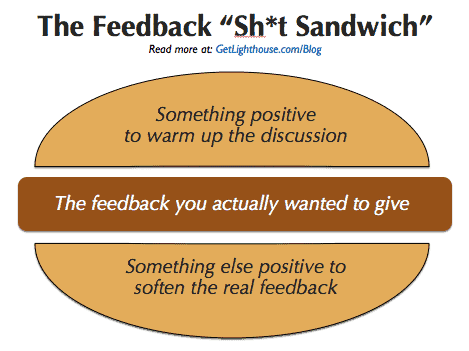
\includegraphics[height=0.9\textheight,width=0.9\textwidth,keepaspectratio]{04_shit_sandwich.png}
\end{frame}
\begin{frame}
    \centering
    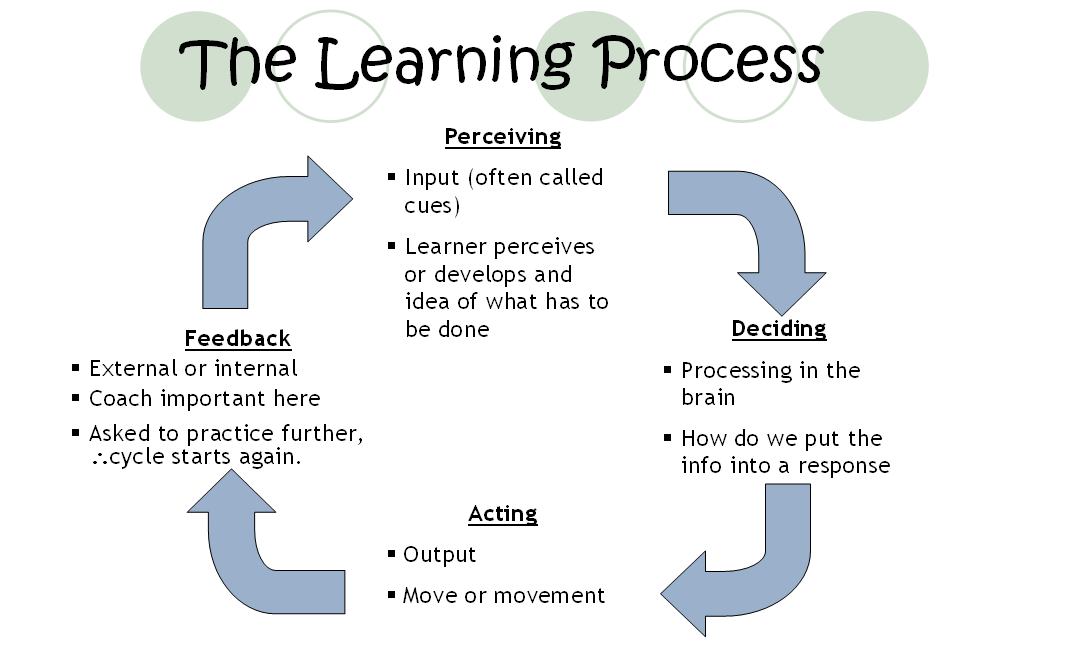
\includegraphics[height=0.8\textheight,width=0.8\textwidth,keepaspectratio]{04_learning_process.png} \footnote{\url{https://clarindabrown.wordpress.com/2011/05/24/a-food-processor-and-the-learning-process/}}
\end{frame}
\begin{frame}{Efficient Learning}
    \begin{itemize}
        \item Why? - Time is precious
        \item How? - Critical and constructive feedback
    \end{itemize}
\end{frame}
\begin{frame}{How can we implement this in engineering teams?}
    \begin{itemize}
        \item Formal debriefs/retrospectives
        \item Informal feedback
    \end{itemize}

    For example:
    \begin{itemize}
        \item Code Reviews
        \item Design Reviews
        \item Expedition/Deployment Debriefs
        \item One-on-one Working Sessions
        \item In the moment feedback
    \end{itemize}
\end{frame}
\begin{frame}{6 R's of Effective Debriefs}
    Reflection

    Reconvene

    Reset

    Review

    Refine

    Recap
\end{frame}
\begin{frame}{Reflection}
    Allows the team to:
    \begin{itemize}
        \item Return from any emotional highs or lows
        \item Individually identify concerns/feedback
    \end{itemize}
\end{frame}
\begin{frame}{Reconvene}
    \begin{itemize}
        \item Set a time
        \item When is too late?
        \item When is too early?
        \item When to decide the time?
    \end{itemize}
\end{frame}
\begin{frame}{Reset}
    \begin{itemize}
        \item No ego, no rank
        \item Reduce authority gradient
        \item Only one role - facilitator
    \end{itemize}
\end{frame}
\begin{frame}{Review}
    \begin{itemize}
        \item Identify objectives/goals
        \item Assess performance
        \item Use context rich stories
        \item Provide feedback
    \end{itemize}
\end{frame}
\begin{frame}{Refine}
    \begin{itemize}
        \item Plan for getting/doing better
        \item Focus on individual and team performance
    \end{itemize}
\end{frame}
\begin{frame}{Recap}
    \begin{itemize}
        \item Review all learnings
        \item Make sure everyone is on the same page
    \end{itemize}
\end{frame}
\begin{frame}{GIFTS}
    Growth Oriented

    I Language

    Functional

    Timely

    Specific
\end{frame}
\begin{frame}{PACE}
    Probe

    Alert

    Challenge

    Emergency
\end{frame}
\begin{frame}
    Activity
\end{frame}
\begin{frame}{Additional Reading}
    \begin{itemize}
        \item \url{https://www.thehumandiver.com/blog/navigating-the-authority-gradient-pt2}
        \item \url{https://www.bjanaesthesia.org.uk/article/S0007-0912(19)30172-2/fulltext}
        \item \url{https://www.mach2consulting.com/wp-content/uploads/2014/01/The-Five-Rs-of-an-Effective-Debrief-Successful-Meetings-Magazine.pdf}
    \end{itemize}
\end{frame}
\end{document}
